\subsubsection{StatefulSet}
\label{subsec:kubernetes:statefulset}
Ähnlich wie Deployments verwalten StatefulSets die Bereitstellung und Skalierung von Pods.
Dabei bietet es eine Garantie für die Reihenfolge und Einzigartigkeit dieser Pods \cite{kubernetesStatefulSets}.
Aufgrund der genannten Garantien werden StatefulSets genutzt, um zustandsabhängige Anwendungen zu verwalten \cite{kubernetesStatefulSets}.
Zur Verwaltung seines Zustands benötigt jeder Pod innerhalb des StatefulSets eigenen Speicher.
Um diesen Speicher für jeden Pod des StatefulSets zu erstellen, muss das StatefulSet dafür sorgen, 
dass jeder Pod ein eigenes \ac{PV} (siehe \ref{subsec:kubernetes:volume}) erhält \cite{Marko2018}.
\begin{figure}[h]
  \centering
  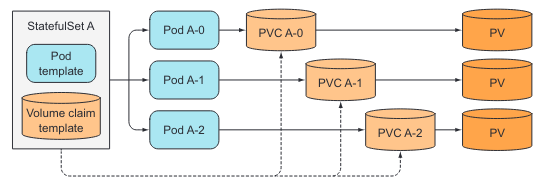
\includegraphics[width=\textwidth]{gfx/chapters/2_grundlagen/statefulsets.png}
  \caption{Zuweisung von Persistent Volumes an Pods in einem StatefulSet}
  \label{fig:kubernetes:statefulsets}
  \source{\cite{Marko2018}}
\end{figure}


In Abbildung \ref{fig:kubernetes:statefulsets} wird dargestellt, wie ein StatefulSet diese Aufgabe übernimmt.
Bei der Erstellung eines StatefulSets muss neben dem Template für die Pods ein \ac{PVC} angegeben werden. 
Dieses \ac{PVC} dient als Grundlage für die Erstellung aller \acp{PV} der Pods \cite{Marko2018}.